%!TEX root = parita-msc.tex
\chapter{Proof Of Concept}
\label{chap:proofOfConcept}
\begin{doublespace}
\par This chapter focuses on some fundamental concepts of \ac{owl} ontologies that were considered while developing the survey instrument for this research work. 
\section{Ontology in Web Semantics}
\par Ontology is a branch of information science that encloses representation, nomenclature, and definition of various properties, categories, and relationships shared among the entities\footnote{includes all types of data, concepts and entities} that support any number of domains the user is interested in. In other words, Ontology is a form of defining a set of concepts for representing the subject properties and the relationships shared among them. According to Tom Gruber~\cite{gruber1995towards}, ontology is \say{an explicit specification of a conceptualization}, where conceptualization is \say{an abstract, simplified view of the world (includes objects, concepts and other entities that are assumed to exist in some area of interest and the relationships that hold among them) that we wish to represent for some purpose}. In web semantics, an ontology is used to define the semantics of the resources briefly and methodically. The ontologies have have been used to \say{specify the physical as well as conceptual characteristics of resources, in the form of metadata schema on the semantic web, for a fixed set of users}~\cite{jacob2003ontologies}.
\section{\ac{owl} Ontologies}
\par W3C developed a standard ontology language called \ac{owl}\footnote{ http://www.w3.org/TR/owl- guide/} to define and describe concepts for ontology using different facilities and operations like intersection, union and negation. It is based on a logical model due to which a reasoner\footnote{maintains hierarchy accurately} can be used to check the mutual consistency among the statements and definitions in the ontology. The reasoner is also responsible for the identification of a suitable concept for particular definitions~\cite{horridge2009practical}.
\subsection{Components of \ac{owl} Ontologies}
\par An \ac{owl} ontology consists of a set of components that define and describe the concepts collectively. The basic components of any \ac{owl} ontology, Individuals, Properties and Classes, are briefly explained in this section.
\begin{itemize}
    \item Individuals:
    \par According to Horridge et al.~\cite{horridge2009practical}, \say{Individuals represent objects in the domain in which we are interested}. Individuals are the objects of classes. Figure~\ref{fig:3.1} shows the representation of different individuals in various domains. The triangles are used here to denote the individuals in free space.
    \begin{figure}[htp]
    \centering
    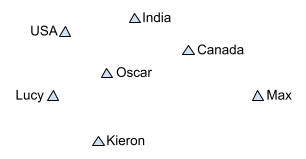
\includegraphics[width=8cm]{images/ch3/Figure1.png}
    \caption{Representation of Individuals in OWL}
    \label{fig:3.1}
\end{figure}
    \item Properties:
    \par The Binary Relationships\footnote{links shared by two individuals} between the individuals (things) are called properties. For instance, the individuals \say{Max} and \say{Kieron} from Figure~\ref{fig:3.1} are linked to each other by the property \say{hasSibling}. Each property can have its inverse. For instance, \say{hasSibling} can have an inverse property \say{isSiblingOf}. The properties can be symmetric or transitive. It is possible to have functional properties where the properties can be restricted to having only one value. Figure~\ref{fig:3.2} shows representation of properties between the individuals \say{Max} and \say{India}, and \say{Max} and \say{hasSibling}. The relation between \say{Max} and \say{India} is \say{livesIn}. The arrow between two individuals in the figure denotes the property (relationship) between them.
    \begin{figure}[htp]
    \centering
    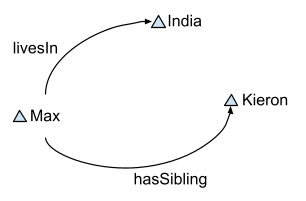
\includegraphics[width=8cm]{images/ch3/Figure2.png}
    \caption{Representation of Properties in OWL}
    \label{fig:3.2}
\end{figure}
    \item Classes:
    \par In \ac{owl}, the sets consisting of individuals are called \ac{owl} classes. Mathematical (formal) descriptions are used to describe the \ac{owl} classes. These descriptions include accurate statements on the requirements for the class membership. For instance, the class \say{Country} consists of all the individuals that are countries in the Domain of Discourse\footnote{can contain one or more classes}. Inheritance in \ac{owl} classes (Class Hierarchy) may exist with the classes having subclasses and/or super-classes which is technically termed as taxonomy. \say{Subclasses specialise (\say{are subsumed by}) their super-classes}~\cite{horridge2009practical}. For instance, consider the classes \say{Lady} and \say{Human}, where \say{Lady} is a subclass of \say{Human}. This implies the following statements:
    \begin{itemize}
        \item All ladies are humans
        \item All members of class \say{Lady} are members of class \say{Human}
        \item Being a \say{Lady} implies that individual is \say{Human}
        \item \say{Lady} is subsumed by \say{Human}
    \end{itemize}
    Figure~\ref{fig:3.3} shows the representation of the classes for the individuals and properties that are shown in Figure~\ref{fig:3.2}.
    \begin{figure}[htp]
    \centering
    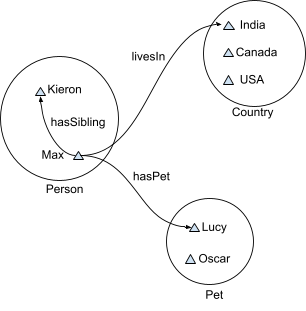
\includegraphics[width=8cm]{images/ch3/Figure3.png}
    \caption{Representation of OWL Classes Consisting of Individuals and Properties}
    \label{fig:3.3}
\end{figure}
\end{itemize}
\section{\ac{owl} Ontology Inconsistencies and Reasoner}
\par A Reasoner\footnote{https://en.wikipedia.org/wiki/Semantic\_reasoner} is used in Protégé to address and solve the inconsistencies. The current version of the Protégé \ac{ide} offers support for some built-in semantic reasoners which are listed below: 
\begin{itemize}
    \item ELK 0.4.3\footnote{https://www.w3.org/2001/sw/wiki/ELK} : A Java-based fast reasoner for lightweight \ac{owl}2 EL which is available under Apache License 2.0
    \item FaCT++ 1.6.5\footnote{https://www.w3.org/2001/sw/wiki/Fact} : A Tableaux-based reasoner for expressive \ac{owl} \ac{dl} which is implemented using C++
    \item HermiT 1.4.3.456\footnote{https://www.w3.org/2001/sw/wiki/Hermit} : A Java-based reasoner, written using \ac{owl}, that can be used to determine consistency of the ontology as well as for the identification of relationships among the classes of the ontology
    \item Mastro DL-Lite\footnote{https://protegewiki.stanford.edu/wiki/Mastro\_DL-Lite\_Reasoner} : An \ac{obda} management system in which the \ac{dl}-Lite family of languages for lightweight \ac{dl} are used for ontology specifications
    \item Ontop 4.1.0\footnote{https://www.w3.org/2001/sw/wiki/Ontop} : A reasoner which uses \ac{sparql} for querying datasets as Virtual \ac{rdf} Graphs
    \item Pellet and Pellet (incremental)\footnote{https://www.w3.org/2001/sw/wiki/Pellet} : A Java-based \ac{owl}2 reasoner for the optimization of nominals, conjunctive query answering, and incremental reasoning
\end{itemize}

\end{doublespace}